To set the stage for what follows in this chapter, we first give a brief overview of some of the concepts in the \AF notation with the help of an example shown in \fig{af:1}.  

The diagram is a simple illustration of a mitogen-activated protein kinase (MAPK) cascade.  The rectangle nodes represent \emph{biological activities} - activities from biological materials, in this case, from macromolecules of proteins (See \sect{af:biologicalActivity}).  Each biological activity can influence, or be influenced by, other biological activities, and such relationships are represented in \AF by lines with arrows and other decorations.  In this particular diagram, all the influences happen to be \emph{positive influences} (See \sect{af:positive_infl}).  The direction of the arrows shows the direction of the activity flow; for example, the RAS activity influences positively (or conventionally called \emph{activates}) the RAF activity.  It should be noted that the essence of \AF is to show the flow of activities from one entity to another or within the same entity.  The underlying mechanisms of how these influences occur are not capture by \AF, but rather, should be described in annotation or captured in other SBGN languages, such \PD and/or \ER. 



\tab{component-summary} summarizes the different SBGN abstractions described in this chapter.

\newcolumntype{P}[1]{>{\raggedright\hspace{0pt}\arraybackslash}p{#1}}

\begin{table}[bh]
  \centering
  \small
  \begin{tabular}{@{}llP{2.4in}P{1.6in}@{}}
    \toprule
    \textbf{Component} & \textbf{Abbrev.} & \textbf{Role} & \textbf{Examples}\\
    \midrule
    Activity node
    & AN
    & ???? 
    & Biological activity \\[0.5em]

    Container node	
    & CN
    & An encapsulation of one or more other SBGN constructs
    & Complexes, compartments \\[1.6em]

    Modulation arc
    & MA
    & Links between different activities to indicate influences.
    & Positive influence, negative influence \\[0.5em]

    Logical operators
    & ---
    & Combines one or several inputs into one output
    & Boolean \emph{and}, \emph{or}, \emph{not} \\
    \bottomrule
  \end{tabular}
  \caption{Summary of \AF components and their roles.}
  \label{tab:component-summary}
\end{table}

\begin{figure}[H]
\centering
\vspace*{-0.75em}
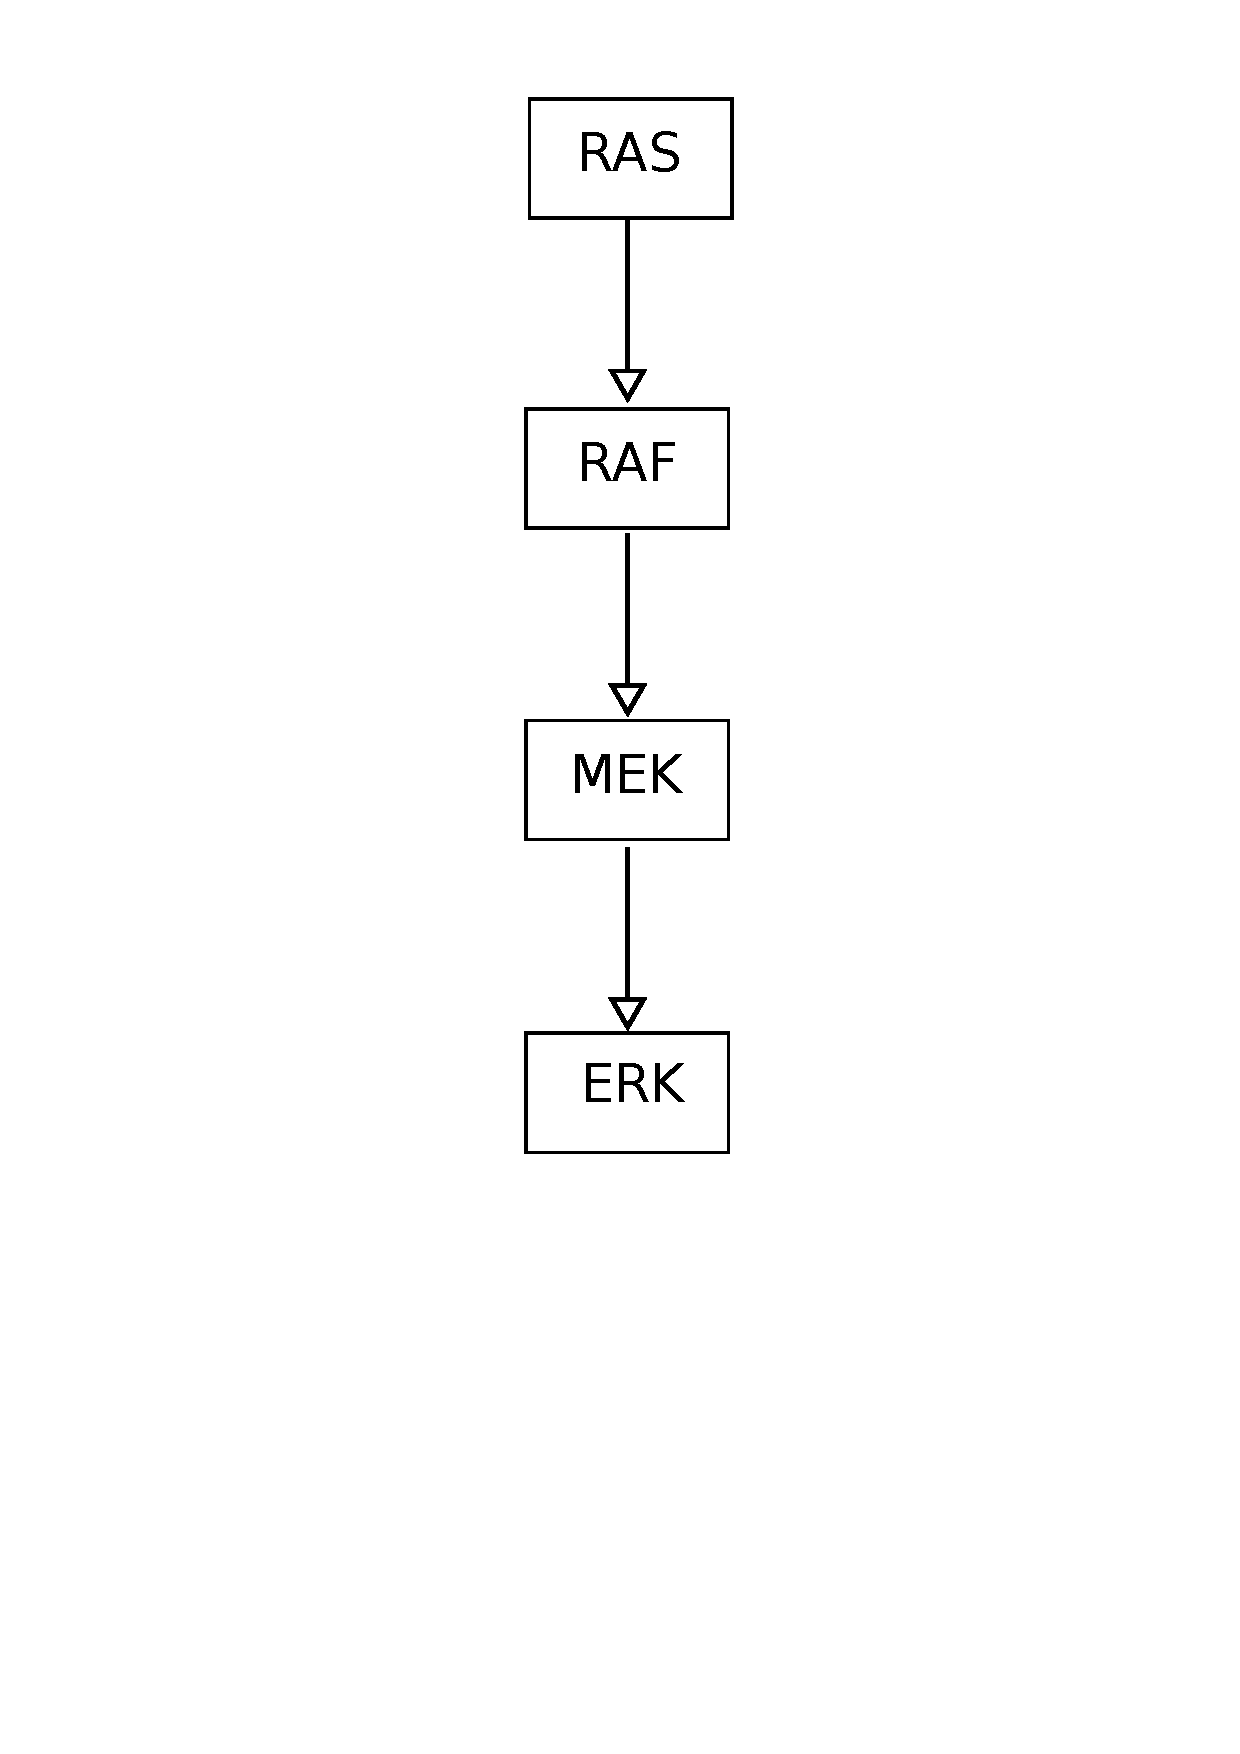
\includegraphics[scale=0.35]{examples/ras-pathway}
\caption{This example of \AF shows two types of symbols: one for activities of different biological materials (\sect{af:biologicalActivity}), in this case, proteins, and another for links between these activities (\sect{af:arcs})}
\label{fig:af:1}
\end{figure}
